\section{Data quality and preprocessing}

All fixes in this section use only the load's own columns or other loads on the same date. None reads the rate, so
they can run before any split without leaking information.

\textbf{Corrupted labels.} For each load we compare its rate per mile with the median of its lane and equipment.
Clean loads sit in a narrow peak. \CorruptRows{} loads (\CorruptPct\%) sit in two separate bands, at about 0.2--0.5
and 2--5 times the lane norm, with almost nothing in between (Figure~\ref{fig:noise}). They appear at the same rate
in every month and equipment type, and no feature predicts them. We treat them as recording errors.

\begin{figure}[H]
  \centering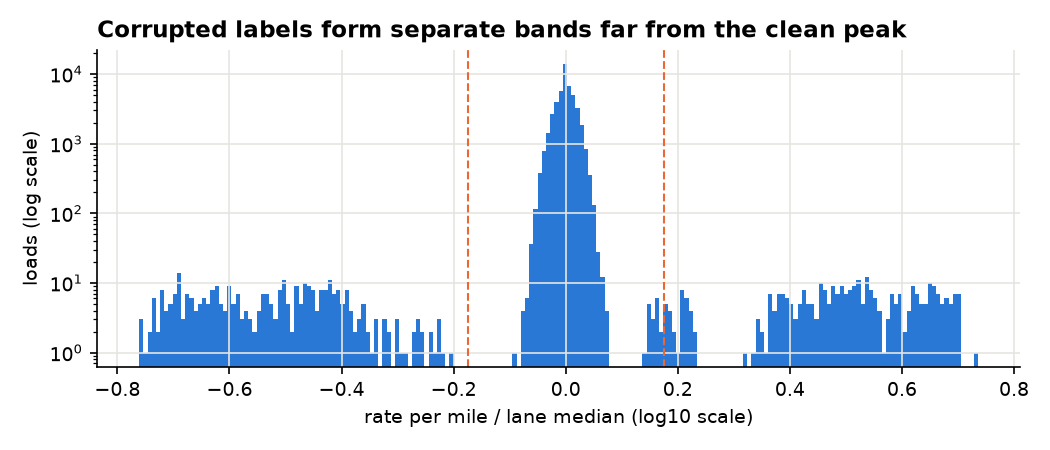
\includegraphics[width=0.8\linewidth]{label_noise.png}
  \caption{Rate per mile relative to the lane median. Dashed lines: the \ScreenLow{} and \ScreenHigh{} screening bounds.}
  \label{fig:noise}
\end{figure}

\emph{Treatment.} Inside every training fold a robust two-pass ridge fit flags rows outside \ScreenLow--\ScreenHigh{} times its
prediction, and those rows are left out of training. The screen is learned, so it never sees assessment rows.
For reporting we use a separate fixed flag (the lane-median ratio above). It marks the same kind of row for every
model and is never used in fitting. Removing the screen costs \usd{\AblNoLabelScreen} on the development folds
(Section~\ref{sec:features}).

\textbf{Negative weights.} \NegativeWeights{} training loads have negative weights whose sizes match normal
weights. These are sign-entry errors, so we use the absolute value.

\textbf{Weight cap.} \CappedWeights{} loads sit exactly at 47,500 lb, a ceiling. A flag tells the model a weight
is capped.

\textbf{Missing values.} \MissingWeights{} weights are missing; we fill them with 31,000 lb (about the median), and
the tree stage sees them as missing. \MissingMarket{} market-index readings are missing; we fill each with that
day's mean, because readings vary little within a day (standard deviation \MarketWithinDaySD) compared with between
days (\MarketBetweenDaySD).

\textbf{Why quote\_signal is dropped.} In training months, \texttt{quote\_signal} either copies the rate per mile
(correlation \QuoteCopyMin{} to \QuoteCopyMax) or mirrors it (\QuoteMirrorMin{} to \QuoteMirrorMax), depending on
the month (Figure~\ref{fig:quote}). In the scoring months that relationship is gone: its correlation with log
distance is \QuoteDistanceCorrValidation, against a typical \QuoteDistanceCorrTrain{} in training. A model that
used it would learn a leak that does not exist when predictions are made. It is never a model input, and a unit
test checks that predictions do not change when it is replaced by noise. Load IDs and city names are not inputs
either.

\begin{figure}[H]
  \centering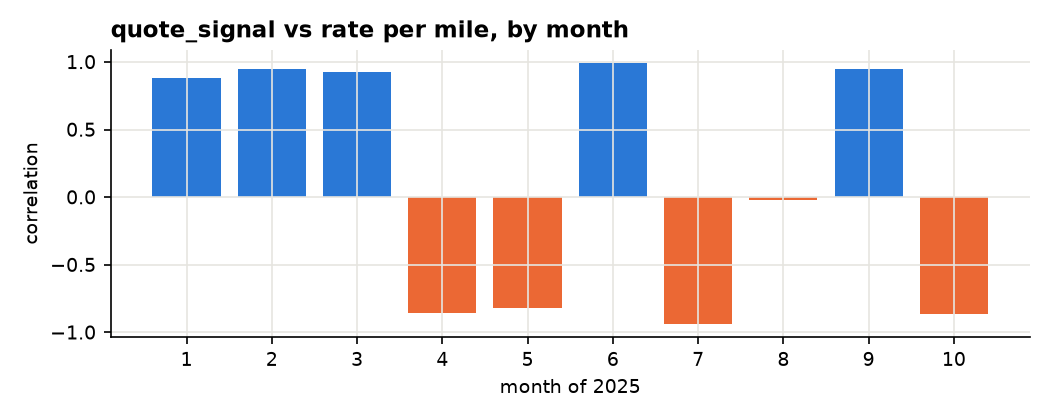
\includegraphics[width=0.8\linewidth]{quote_signal.png}
  \caption{Monthly correlation of \texttt{quote\_signal} with the rate per mile (clean training rows).}
  \label{fig:quote}
\end{figure}
